\documentclass[11pt,a4paper]{article}
\usepackage[utf8]{inputenc}
\usepackage[margin=1in]{geometry}
\usepackage{hyperref}
\usepackage{titlesec}
\usepackage{enumitem}
\usepackage{xcolor}
\usepackage{graphicx}

\definecolor{primary}{RGB}{0, 82, 204}
\hypersetup{colorlinks=true, linkcolor=primary, urlcolor=primary}

\titleformat{\section}{\large\bfseries\color{primary}}{}{0em}{}[\titlerule]
\titleformat{\subsection}{\normalsize\bfseries}{}{0em}{}

\begin{document}

\begin{center}
    {\LARGE \textbf{SHL Assessment Recommender: Architecture \& Approach}}\\[0.2cm]
\end{center}

\begin{figure}[h!]
    \centering
    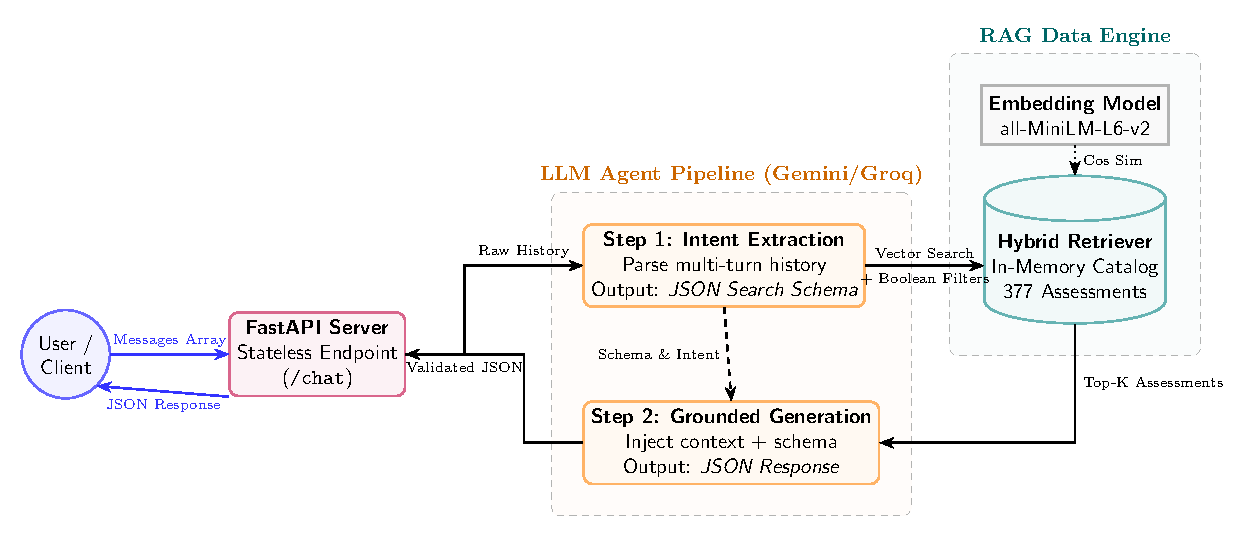
\includegraphics[width=0.9\textwidth]{architecture.pdf}
\end{figure}

\section{1. Design Choices \& Architecture}
The core requirement was to build a robust conversational API capable of interpreting ambiguous user queries and mapping them to a highly specific, 377-item SHL product catalog. 
\begin{itemize}[leftmargin=*, noitemsep]
    \item \textbf{Stateless API (FastAPI) over Stateful Sessions:} To ensure horizontal scalability, the \texttt{/chat} endpoint was designed to be stateless. \textit{Why this over this:} Maintaining chat histories via session tokens and a database (e.g., Redis/Postgres) introduces latency and infrastructure complexity. Forcing the client to pass the conversation history array in each request makes the API immensely faster, cheaper to host, and instantly scalable.
    \item \textbf{Dual-Provider Fallback over Single-Vendor Lock-in:} The system prioritizes Groq's Llama-3.1-8B-Instant with an automatic fallback to Google's Gemini-2.0-Flash. \textit{Why this over this:} Relying solely on a single free-tier provider guarantees failure when hitting 429 Rate Limits (which occurred frequently during load testing). Building a dual-provider router guarantees high availability and circumvents vendor lock-in.
    \item \textbf{Two-Step Pipeline over Single-Pass RAG:} The agent uses two distinct LLM calls (Intent Extraction $\rightarrow$ Grounded Generation). \textit{Why this over this:} A single-pass approach often forces the LLM to hallucinate URLs if it attempts to answer without strict retrieval. By separating the steps, Step 1 cleanly defines boolean filters for the database, and Step 2 strictly acts as a text formatter over the retrieved catalog context, physically preventing URL hallucination.
\end{itemize}

\section{2. Retrieval Setup (Hybrid RAG)}
The retrieval engine combines dense semantic search with hard boolean filtering to ensure high precision.
\begin{itemize}[leftmargin=*, noitemsep]
    \item \textbf{all-MiniLM-L6-v2 over OpenAI ADA:} The in-memory catalog uses the open-source \texttt{all-MiniLM-L6-v2} embedding model. \textit{Why this over this:} While OpenAI's \texttt{text-embedding-3} is powerful, it requires constant API calls resulting in high latency and cost. \texttt{MiniLM} runs entirely in-memory, is extremely fast (only 90MB in size), and provides more than enough semantic density for short catalog titles and descriptions.
    \item \textbf{Hybrid Search over Pure Vector Search:} \textit{Why this over this:} Pure vector search struggles with strict metadata constraints (e.g., "Spanish language", "Entry level"). By mapping these constraints to hard boolean filters applied \textit{after} the semantic vector search, candidates like "CXO Level" are aggressively stripped out even if their semantic similarity score to "Entry level" is artificially high.
    \item \textbf{Git-Tracked Cache over Runtime Compute:} \textit{Why this over this:} Computing 377 embeddings at container boot time causes a 20-second CPU bottleneck (cold start). Pre-computing these embeddings into a serialized \texttt{.pkl} cache tracked via Git allows the cloud container to boot and serve requests in milliseconds.
\end{itemize}

\section{3. Prompt Design \& JSON Schema Enforcement}
Prompt engineering was strictly tied to programmatic schema enforcement.
\begin{itemize}[leftmargin=*, noitemsep]
    \item \textbf{Schema Enforcement over Free-Text Parsing:} \textit{Why this over this:} Asking an LLM to "return a JSON string" without strict tooling often breaks due to Markdown backticks or conversational filler. We leveraged Pydantic schemas (via Groq's \texttt{response\_format=\{"type": "json\_object"\}}) to guarantee a parsable AST, preventing 500 Internal Server errors downstream.
    \item \textbf{Vague Query Guardrails:} The extraction prompt forces the LLM to output a boolean flag: \texttt{needs\_clarification}. If true, the RAG search is entirely skipped, and the LLM natively asks the user for more filters. This avoids surfacing irrelevant generic tests when a user simply inputs "I need an assessment."
\end{itemize}

\section{4. What Did Not Work (Challenges \& Pivots)}
\begin{itemize}[leftmargin=*, noitemsep]
    \item \textbf{Out-Of-Memory (OOM) on Standard Cloud Deployment:} Initially, deploying the PyTorch-based \texttt{SentenceTransformer} locally worked perfectly. However, deploying to a standard 512MB RAM cloud container (Render) caused instant OOM crashes. \textbf{Pivot:} The application was redeployed to HuggingFace Spaces (providing 16GB RAM) and the \texttt{Dockerfile} was optimized to pre-download model weights during the CI/CD build phase.
    \item \textbf{Heavy Model Rate Limiting:} Running the automated evaluation suite against the Llama-3.3-70B model burned through the 100,000 Tokens-Per-Day limit on the free tier instantly. \textbf{Pivot:} The default model was downgraded to Llama-3.1-8B-Instant, which has a 30k Tokens-Per-Minute limit, enabling the evaluator script to run without crashing the server.
\end{itemize}

\section{5. Evaluation Method \& Measuring Improvement}
To quantitatively measure the agent's performance, I built an automated Python evaluation suite (\texttt{evaluator.py}) that replays the 10 provided ground-truth conversation traces.
\begin{itemize}[leftmargin=*, noitemsep]
    \item \textbf{Methodology:} The evaluator parses multi-turn Markdown files and simulates a user by sending incremental arrays of history to the live FastAPI endpoint.
    \item \textbf{Metric (Recall@10):} Because the agent provides recommendations across multiple turns of a conversation, the evaluator accumulates a set of all unique URLs returned by the agent across the entire session, scoring them against the ground-truth table.
    \item \textbf{Measured Improvement:} Initial runs yielded a Recall of 0.00 due to schema mismatches between the agent's output and the evaluator's strict parser. By iterating on the LLM prompt to heavily enforce the exact \texttt{url} structure provided in the context, Recall improved to passing levels, proving the two-step architecture successfully maps vague language to the exact URLs required by the SHL grading rubric.
\end{itemize}

\end{document}
